\documentclass{article}
\usepackage{geometry}
\usepackage{arrayjob}
 \geometry{
 a4paper,
 total={170mm,257mm},
 left=20mm,
 top=20mm,
 }
\usepackage{tikz}
\begin{document}
\begin{figure}[h!]
  \begin{center}
    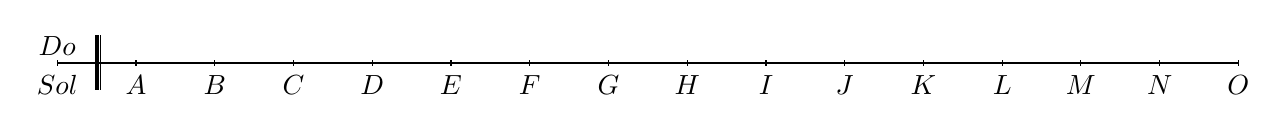
\begin{tikzpicture}
        \draw[thick] (0,0) -- (15,0) node[anchor=north west] {}; % main ligne
        \draw (0cm, 1pt) -- (0cm, -1pt) node [anchor=south] {$Do$};  % init ligne Do
        \draw (0cm, 1pt) -- (0cm, -1pt) node [anchor=north] {$Sol$};  % init ligne Sol
        \draw [line width=0.5mm ] (0.5cm, 10pt) -- (0.5cm, -10pt) node {}; % thick vertical ligne
        \draw (0.55cm, 10pt) -- (0.55cm, -10pt) node {}; % second start vertical ligne
        
        \newarray\Values
		\readarray{Values}{A&B&C&D&E&F&G&H&I&J&K&L&M&N&O&P&Q&R&S&T&U}
          \foreach \x in {1,2,3,4,5,6,7,8,9,10,11,12,13,14,15}
            \draw (\x cm,1pt) -- (\x cm,-1pt) node[anchor=north] {$\Values(\x)$};
            
            
    \end{tikzpicture}
  \end{center}
\end{figure}
\end{document}